\documentclass[12pt]{article}

\usepackage[a4paper, margin=1in]{geometry}
\usepackage{graphicx}
\usepackage[absolute, overlay]{textpos}
\usepackage{fancyhdr}
\usepackage{siunitx}
\usepackage{tikz}
\usepackage{pgfplots}
\usetikzlibrary{decorations.pathmorphing}
\usetikzlibrary{math}
\usetikzlibrary{calc}

\pgfplotsset{compat=1.18}

\pagestyle{fancy} %for footers

\newcommand{\customsubject}{}   
\newcommand{\customtitle}{}

\newcounter{questionpartcounter}                  %Setup for question part counter for a,b,c listing
\renewcommand{\thequestionpartcounter}
{\alph{questionpartcounter}}

\newcounter{questionpartpartcounter}                  %Setup for question part  partcounter for a,b,c listing
\renewcommand{\thequestionpartpartcounter}
{\roman{questionpartcounter}}

\pagestyle{fancy} %for footers
\renewcommand{\headrulewidth}{0pt}
\fancyhf{}
\fancyfoot[R]{\thepage}

\newenvironment{worksheet}[2]
{
    
    \global\renewcommand{\customtitle}{#1}
    \global\renewcommand{\customsubject}{#2}


    \begin{textblock*}{5cm}(0.4cm,0.4cm)
   
\includegraphics[width=4cm]{include/figures/bmdwlogo}
\end{textblock*}

    \vspace*{-1cm}
    
    {\large\textbf{\begin{center}\customtitle\end{center}}}

    \begin{center}\customsubject\end{center}
    
    \vspace{0.3cm}
    
    \hspace*{-1.5cm}\textbf{Name:\ \rule{4cm}{0.4pt}}\; 
    \textbf{Student \#: \ \rule{3cm}{0.4pt}}\;
    \textbf{Student Email \#: \ \rule{1.53cm}{0.4pt}}

    \vspace{0.5cm}

    
    \begin{enumerate}
}
{
    \end{enumerate}
   % \begin{textblock*}{10cm}(1cm, 28cm) {\footnotesize \scriptsize \customsubject}
    
%\end{textblock*}
}



\newcommand{\question}[2][1cm]{%
    \item
    \setcounter{questionpartcounter}{0}
    \setcounter{questionpartpartcounter}{0}
    {#2}
    \vspace{#1}
}

\newcommand{\questionpart}[2][1cm]{%
    \setcounter{questionpartpartcounter}{0}
    \stepcounter{questionpartcounter}
    (\thequestionpartcounter)~#2
    \vspace{#1}
}

\newcommand{\questionpartpart}[2][1cm]{%
      \stepcounter{questionpartpartcounter}
      \thequestionpartpartcounter.~#2
      \vspace{#1}
}

\newcommand{\operation}[1]{%
{\large $
#1
$}
}



\begin{document}

\begin{worksheet}{Physics Worksheet}{Vectors}

\question[2cm]{Algebra With Vectors}{A boat is traveling across a river. It's going south east with a velocity of: \\ $\vec{v_B} = (-5,-4) \si{\kilo\metre\per\hour}$. The river is flowing with a velocity of  $\vec{v_w} = (2,1) \si{\kilo\metre\per\hour}$. With what velocity is the boat crossing the river?}

\question[2cm]{Scalar Product}{Aki and Luke go running off in different directions. $\vec{v_A}= (\frac{1}{3},2) \si{\metre\per\second}, \\ \vec{v_L}= (-1,\frac{3}{4})\si{\metre\per\second}$. What is the angle between their velocity vectors?}

\question[3cm]{Cross Product}{A force $\vec{F} = (6,3)$ is applied to the edge of a disc centered at the origin at $\vec{r} = (1,2)$. What is the magnitude and direction of the angular acceleration?
\\
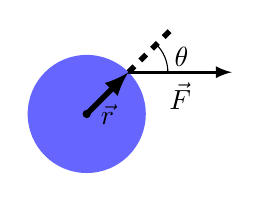
\begin{tikzpicture}[scale=1]
\tikzmath{
\R=0.75;
}
\scalebox{1.0}{

\fill[color=blue!60] circle (\R);
\fill[black] circle (1.5pt);

\draw[-latex, line width = 2pt] (0,0) -- (45:\R) node[midway, below]{$\vec r$};
\draw[dashed, line width = 2pt] (45:\R) -- + (45:\R);
\draw ($(45:\R)+(0.5,0)$) arc (0:45:0.5) node[midway, right]{$\theta$};
\draw[-latex, line width = 1pt] (45:\R) -- + (1.75*\R,0) node[midway, below]{$\vec F$};

}
\end{tikzpicture}}

\question{Right Hand Rule}{Insert questions and tikz drawings here}

\end{worksheet}


\end{document}